% We now introduce three case studies, \ie product lines that (can) jeopardize trade secrets.
% For each case, we describe (1) the application domain, the management of variability, and the economical value of the product line; (2) the trade secrets a product line can incidentally jeopardize due to improper management and implementation of variability. 
% Section~\ref{sec:summary} will further discuss the underlying challenges for protecting product lines and their variability.
% As we will see, the video service is representative of the product line issues identified in the introduction; it acts as a case study~\cite{yin2002}.
% (i.e., "an empirical inquiry that investigates a contemporary phenomenon within its real-life context"~\cite{yin2002}).


\subsection{Online Newspapers (Cont')}
\label{sec:casestudy1}
\input{newspaper.tex}

\dcs
% We consider again the case of online newspapers. 
 The first example in the introduction is based on a real wrong design decision\footnote{\url{http://linuxfr.org/users/jarvis/journaux/lemonde-fr-ou-l-abonnement-au-javascript}} that has been fixed afterwards. % ~\cite{linuxfr}
We now describe another problem in the same domain. For confidential reasons, we call it \textsf{\fakenewspaper} hereafter. % we do not mention the name of the newspaper. We 
% 
 The website is separated in two domains (1) 
% \begin{itemize}
% \item 
www.\fakenewspaper.\\com gives a limited access to public articles;
% \item 
 (2) subscribers.\\ \fakenewspaper.com gives a complete access to paying customers.
% \end{itemize}
In complement to providing early access to new articles, the variant of \textsf{\fakenewspaper} for subscribers provides additional services (e.g., easy-reading option, limited amount of advertising). % innovative navigation, better interfaces for mobile supports, 
% (\emph{plus} some services like easy-reading). 
 As in the previous example, the verification is done on the client side. 
When a visitor accesses subscribers.\fakenewspaper.com, a JavaScript checks whether she is a member. 
In case the user is not a member, the page is redirected to www.\fakenewspaper.com. 

\wprv
By deactivating JavaScript\footnote{\eg with \url{https://noscript.net/}}, a regular (non paying) reader can  access articles that should be restricted to subscribers.\fakenewspaper.com. 
An outsider can even implement a script that automates the task of finding the complete text in subscribers.\fakenewspaper.com and injecting it in the normal page of www.\fakenewspaper.com:
 \lstinputlisting[language=javascript, firstline=1]{lemonde2.js}
Similar scripts can be implemented so that regular readers can use the variant of \fakenewspaper and benefit from the subscribers' options (e.g., limited advertising) of subscribers.\fakenewspaper.com  for free. 

We can wonder why \textsf{\fakenewspaper} uses such a naive approach for protecting its variant and options. 
Several hypothesis can be formulated. The first one is that this approach is easy to implement for developers while the economical risk might be considered as limited. That is, there is a tradeoff between development effort and protection of trade secrets. 
The second hypothesis is that there is actually a third variant for Web search engines. There is a clear need to reference content in this domain -- it is crucial for the business of newspapers to be properly referenced in search engines. This implementation strategy has the merit of allowing search engines to easily crawl the articles. 
Again a tradeoff has certainly been discussed and found. In any case, the current solution is clearly suboptimal. 
More sophisticated strategies can certainly be considered not to jeopardize trade secrets. 
%  find. 
% there is a tradeoff 


\vspace*{-2mm}
\subsection{Video Generator}
\label{sec:casestudy2}




\dcs
We report on an experience related to an online video generator. 
% Some details have been reported in. % (\url{http://bref30ans.canalplus.fr}). 
 Compared to~\cite{BrefVamos14}, we add here further details under the angle of software protection.
% The goal is to explain that the video service is representative of the product line issues identified in the introduction; it acts as a case study~\cite{yin2002}.
% (i.e., "an empirical inquiry that investigates a contemporary phenomenon within its real-life context"~\cite{yin2002}).
 The service offers to generate variants of an humorous video. Internet users simply have to type their name, select 3 options, and a particular video is launched and visualised in the browser. % (see Figure~\ref{fig:brefo}, page~\pageref{fig:brefo}). 
The service is quite popular and successful: more than 1.7M of video variants have been generated in 1 week. 
%We had an interest in the Web site, since the service claims that a particular video is resulting from a combination among billions. Moreover the term % \emph{generator} is explicitly employed.  
% Our original intuition was that the video service resembles to a software product line, i.e., generative techniques and variability are likely to be present. 
 We put ourselves as attackers. We audited and studied the generator as a black box system without access to the source code of the server side. 
% Moreover, client side code is obfuscated as in the original service. 
%A first step was to reverse engineer the system. 
% In essence, reverse engineering \emph{"consists in deriving information from the available software artifacts and translating it into abstract representations more easily understandable by humans"}~\cite{canfora2011}. 
 We started reverse engineering the service through the analysis of the communications between the server and the client. 
Though the JavaScript was \emph{obfuscated}, the observations of HTTP requests and the use of a JavaScript debugger reveal the overall behaviour. We quickly noticed that all video variants are constituted of 18 sequences of videos that are themselves separated in several sub-parts. 
That is, a video variant is modularized. 


% \vspace*{-2mm}

The partitioning of the video in 18 sequences forms a first level of modularity (see \ding{192} in Figure~\ref{fig:generator}). % The objective is to avoid the generation of billions of videos on the server side.
For each sequence of a video, numerous alternatives are possible. This corresponds to a second level of modularity which focus on the variability of the video sequences (see \ding{193} in Figure~\ref{fig:generator}). A video variant results of the selection of an alternative for each sequence. The generator automatically selects an alternative, either based on the 3 selected options or through probabilistic choices for the other 15 sequences. 
% (the inference of frequencies per alternatives is out of the scope of the paper).
 Finally, a third level of modularity is realized by the partitioning of each alternative (see \ding{194} in Figure~\ref{fig:generator}). Overall modularity allows the server to share small video files and thus to improve the scalability/reactivity the service.
 
 
\begin{figure}
\centering
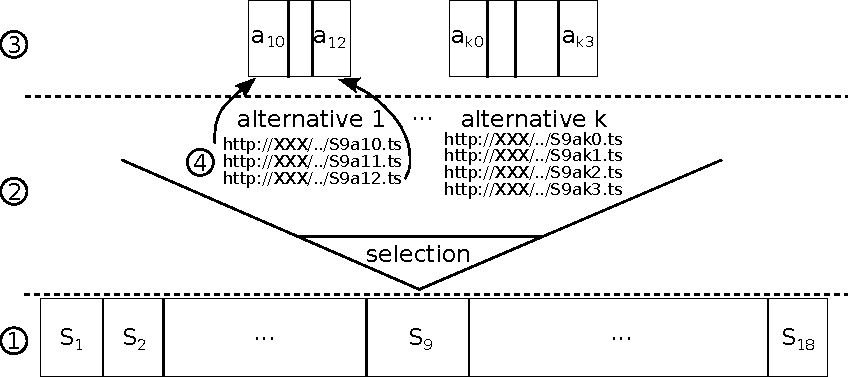
\includegraphics[width=1\linewidth]{figures/bref-generator.pdf}
\vspace*{-4mm}
\caption{\label{fig:generator}Video generator: modularity and variants}
% \vspace*{-4mm}
\end{figure}

Figure~\ref{fig:process} shows how the client and the server communicate to generate and play a video variant. First, the client asks for the generation of a new video. The server returns a list of file names corresponding to the selected sequences ($\{S1a2, ..., S18a4\}$ in our example).  
Each file corresponds to a playlist that defines the sub-parts of the sequence \eg in \ding{195} of Figure~\ref{fig:generator} the playlist defines 3 sub-videos: S9a10, S9a11 and S9a12.
The client downloads all the playlists and their corresponding videos. Finally, the client \emph{merges} the videos of the playlists and plays the resulting video variant.


\begin{figure}
\centering
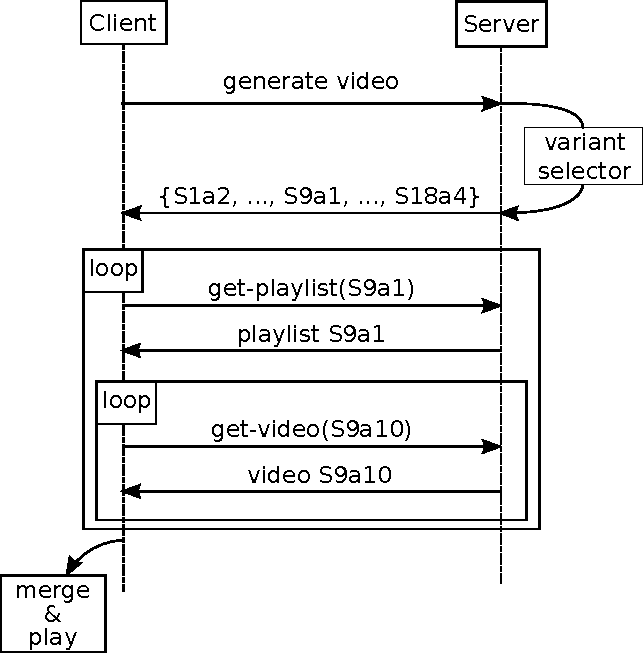
\includegraphics[width=0.7\linewidth]{figures/server-client.pdf}
\vspace*{-2mm}
\caption{\label{fig:process}Communications server/client}
\vspace*{-4mm}
\end{figure}





% We have then contacted the creators of the video generator with two research questions and goals in mind: (1) can we \emph{automate} the extraction of variation points and configurations (video variants)? (2) can we re-engineer another generator and configurator? 
% The creators accepted to collaborate and provided us with an access to an offline version of the generator. However we did not have access to the source code % neither in the server side nor in the client side. Like this, we can study the generator as a black box system -- as it would be the case in reality -- but without disturbing the deployed Web generator (e.g., with hundreds of HTTP requests). 
% \ma{We can remove this one: 
% The interest for the creators was to audit their systems.
 % security mechanisms for avoiding or at least complicating our tasks.
%




%  and defensive mechanisms have to be considered. 

\wprv
%
%  Our first audit showed that a reverse engineering work can get access to all the video sequences. Furthermore, ,
   % (see~\cite{BrefVamos14} for more details). 
% 15 new variation points are now apparent, out of which 13 are configurable (i.e., exhibiting at least 2 alternatives). 
% For the 3 variation points also present in the original configurator, users can now explicitly choose the alternatives. 
 The implementation of the product line can cause two important threats. 
The first threat is that an attacker can download the video sequences, which are protected by copyright. As digital content is a key business value, protecting the access to data becomes a security problem. Without defensive mechanisms, an attacker can extract and generate all the possible video variants of the original service. 
%
 The second consequence is that a new configurator can be re-engineered and could "kill the original idea"~\cite{BrefVamos14}. Specifically we showed it is straightforward to re-engineer a new generator and configurator in which users configure in a fine-grained way the 18 variations points -- instead of only 3 in the original version.
That is, with a re-engineered solution, the surprise effect is limited when getting a new video variant. Instead, users can control, choose and visualize \emph{any} alternative (video sequence). The creators of the generator did not have this intention  -- they did not want to jeopardize their trade secrets.

% calling to consider security issues. % -- though the idea of  
% -- thus dramatically limiting the \emph{surprise} effect. 

 % In other words, they have taken a strategic decision for, on-purpose, delimiting the scope of variability and restraining the visibility of some variation points and alternatives. 

% Our experience shows that the scoping of variability (i.e., what is visible to users) is a strategic solution and, 
% Overall the generator is well engineered and modularity is the right way to do from a development perspective. 
% Modularity is also needed to scale: as further emphasized in the next section, it is technically difficult to pre-generate millions of video variants.   \ma{says something like "modularity" or "featurization" is advocated by SPLE}

An important lesson learned is that the \emph{modularity} of data (video variants) poses a problem from a protection perspective.  
From a software engineering and product line perspective, modularity is undeniably good and remains a standing goal of any project. However modularity can backfire: an attacker can too easily understand the generation process and the differences between alternative sequences. 
With modularity, the task of determining the number of sequences and identifying the alternatives corresponding to each sequence does not face any obstacles. Similarly the collection and the \emph{composition} of video sequences is immediately understood. 
% Overall, a malicious attacker could not only collect all videos but could also launch a new competing video generator service; it is not acceptable.

Another important lesson learned is that an attacker should have difficulties to navigate into the configuration space. Otherwise she will be able to understand the whole product line and extract trade secrets in a \emph{comprehensive} and \emph{automatic} manner. Protection mechanisms for blocking frequent requests are worth considering but may not be sufficient. 
% An attacker can have difficulties to explore the modularity space.

 
% \ma{insist more on the "configurations" problem; rephrase or insist more on the "variability" aspect}




% \subsection{Windows Operating System Family}
% \label{sec:casestudy3}
% \dcs
%
 We describe some hacks related to the family of Windows operating systems. Microsoft sold its Windows products in three distinct packages: (1) \emph{full packaged product} is intended for installation on computers that have not previously had a licensed copy of the software; \emph{upgrade packages} offer a discount to owners of a previous edition of a given product; 
% In virtually all cases, the license terms require that you stop using the previous edition.
 (3) \emph{original equipment manufacturer} products offer the steepest discounts of all and are installed on new or refurbished computers.
% \end{itemize}

In 2008, an upgrade hack in Windows Vista allowed end users to purchase the upgrade edition and install it on any computer -- with no need to purchase the more expensive full edition. Interestingly, the upgrade disc contained in fact the \emph{whole} product line (\ie not just an upgrade).
%

In 2009, Windows 7 was subject to a hack that allows a clean install of the operating system using an upgrade disc rather than the full version upgrades~\cite{w7microsoft}. 
Eric Ligman, Microsoft senior sales excellence manager, wrote a series of blog posts. 
He recognized the hack but also warned users about licensing issues:
\begin{quote}
Over the past several days there have been various posts, etc. across a variety of social media engines stating that some "hack" shows that a Windows 7 Upgrade disc can perform a "clean" installation of Windows 7 on a blank drive from a technical perspective. 
Of course, from the posts I saw, they often forgot to mention a very basic, yet very important piece of information... "Technically possible" does not always mean legal. 
\end{quote} 
 % version 
% Some proprietary systems or applications hide on purpose some features. Users typically have to pay for activating the features. For example, 
% It calls for investigating \emph{variability-aware security} mechanisms. 

In 2014, Microsoft announced to stop supporting Windows XP, but a simple registry hack lets users continue to get security updates.
The registry setting makes Windows Update thinks Windows XP system is actually Windows XP POSReady (which is still supported). 
Hence a Windows XP machine can receive updates for another five years. %, without having to pay. 
Microsoft quickly reacted: 
\begin{quote}
% We recently became aware of a hack that purportedly aims to provide security updates to Windows XP customers. 
The security updates that could be installed are intended for Windows Embedded and Windows Server 2003 customers and do not fully protect Windows XP customers. Windows XP customers also run a significant risk of functionality issues with their machines if they install these updates, as they are not tested against Windows XP.
\end{quote}


\wprv
% 
 The stories with the different variants of Windows have some consequences. Users without a full license of Windows (e.g., Windows 7 Beta available during the trial phases) can fully install Windows 7. Users can apply continued security updates for Windows XP (despite the end of the support).
The naive implementation allows outsiders to easily modify the settings of the product line. The case shows that technical hacks may be employed to bypass Windows. Though all workarounds violate the terms of license agreements, Microsoft was forced to quickly react and communicate.  

 

\subsection{Web Configurators}
\label{sec:casestudy4}
\dcs
%
 % In many markets, organisations are competing to propose customised products, characterised by hundreds of inter-related \textit{configuration options}. 
 % As the repertoire of inter-related options can be disconcerting for many customers, \textit{Web configurators} are developed to assist them during decision making.
% As an example, Figure~\ref{fig:configurationDummy} shows a snapshot of a typical car configurator (the circled letters and legend can be ignored for now). 
 A Web configurator provides an interactive graphical user interface that guides the users through the configuration process, verifies constraints between options, propagates user decisions, and handles conflictual decisions~\cite{ebrahimCSMR2014}. %ebrahim2013}. %rogoll2004,streichsbier2009,Trentin2012}.
% Configurators are used in many applications to personalize products and services. 
 Configurators are used in installation wizards, preference managers, and extensively used in product lines. 
 %  
 The database maintained by Cyledge is a striking evidence with 900+ Web configurators coming from 30+ different industry sectors~\cite{configurators}. % ~\cite{configurators}
% \footnote{\url{http://www.configurator-database.com}}

% Since 2007, Cyledge collected more than 900 Web configurators coming from 30+ different industry sectors, including automotive, apparel, sport, and art. 
% 
 A very simple excerpt of a real-world Web configurator is depicted in the Figure below. % ~\ref{fig:configurationDummy}. 
We can observe that the selection of \textsf{Diesel} has lead to the automated selection of \textsf{EDC6}. (In fact, some other equipment options have been previously selected; one can select \textsf{Diesel} with \textsf{EDC7} or \textsf{BVM} in some other configuration settings.) 
That is, a customer has not chosen \textsf{EDC6}; the configurator has imposed some constraints of different natures: technical/engineering constraints, aesthetic constraints, marketing constraints, \etc


% \begin{figure}[!hts]
% \vspace*{-3mm}
% \begin{center}
% \includegraphics[scale=0.31]{img/configuratorDummy.png}
%   \vspace*{-7mm}
% \caption{Audi web SC (\texttt{http://configurator.audi.co.uk/}, Oct. 18, 2012)} %\url{
% \vspace*{-9mm}
% \label{fig:configurationDummy}
% \end{center}
% \end{figure}

\begin{figure}[!ht]
\centering
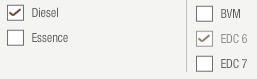
\includegraphics[scale=0.5]{figures/configuratorRenault.png}
% \vspace*{-2mm}
%\caption{{\small{Options and constraints in a configurator}}} 
% \label{fig:configurationDummy}
\vspace*{-2mm}
\end{figure}


% SCs represent a significant portion of the configurators used in modern information systems. %Their application domains range from y are used to automate the tuning of information systems to the preferences of the user. Installation wizards, preferences managers, and configurable business process models~\cite{quteprints12686,DBLP:conf/caise/GottschalkWJAR09} are examples thereof. 

% where multiple information system variants are derived from a base of reusable artefacts according to the specific characteristics of the targeted customer or market segment~\cite{Pohl2005,Schaler:2012:BIS:2363463.2363516,DBLP:conf/caise/GottschalkWJAR09,quteprints12686}. 

% A significant share of existing configurators is Web-based, irrespective of the market. 

% In this paper, we focus on web configurators supporting online sales.%, but we will argue that some of our findings generalize to other types of configurators.




% These configurators vary significantly. They each have their own characteristics, spanning visual
% aspects (GUI elements) to constraint management. 
% The web SC of Audi appearing in Figure~\ref{fig:configurationDummy} is thus only one example. It displays different options through specific widgets (radio buttons and check boxes -- \textcolor{red}{ \mycirc{A}} and \textcolor{red}{\mycirc{B}}, respectively). These options can be in different states such as activated (e.g., \configopt{Privacy glass} is flagged with \checkmark) or unavailable (e.g., \configopt{Twin-pane UV and heat-insulating glass} is greyed out). Additionally, these options are organised in different tabs (e.g., \configopt{Equipment}) and sub-tabs (e.g., \configopt{Equipment packages}) which denote a series of steps (\textcolor{red}{\mycirc{C}}) in the \emph{configuration process} (e.g., \configopt{1. Model} is followed by \configopt{2. Engine}-- \textcolor{red}{\mycirc{D}}). A SC can also implement \emph{cross-cutting\footnote{We call these constraints \emph{cross-cutting} because they are often orthogonal to the hierarchy of options, sub-options, etc. supported by the configurator.} constraints} between options (\textcolor{red}{\mycirc{E}}). These are usually hidden to the user but they determine valid combinations of options. For instance, the selection of \configopt{Privacy glass} implies the deselection of \configopt{Twin-pane UV and heat-insulating glass}, meaning that the user cannot select the latter if the former is selected. 
% Moreover, descriptive information (\textcolor{red}{\mycirc{F}}) is sometimes associated to an option (e.g., its price). % of the product.

\wprv
% As privileged channels for identifying customer needs and placing orders, configurators are key assets for companies. 
 Products, options, and the underlying constraints a configurator is in charge of are key information of an organization. 
Such information is particularly interesting from the perspective of (online) \emph{market intelligence (MI)} (also called \emph{competitive intelligence}). 
MI can be defined as the "information relevant to a company's
markets, gathered and analyzed specifically for the purpose of accurate and confident decision-making in determining
market opportunity, market penetration strategy, and market development metrics." 
Lixto, a company offering data extraction tools and services for MI, showed that it is technically feasible to acquire and exploit unstructured and semi-structured data in several case studies (\eg in the domain of computers and electronics consumer goods~\cite{baumgartner2009}). % 

Most information on pricing, product availability, product options, and product constraints is potentially available on Web sales configurators.
Specifically, competitors can use this information (1) for getting a comprehensive overview of the options and constraints in the market; (2) to be (continually) informed about strengths and weaknesses of other competitors' product lines; (3) to publicly reveal a certain superiority or marketing practice, \etc
  
 Web data extraction systems~\cite{baumgartner2009,Ferrara2014} can be specialized for acquiring configurators' information. 
 Early attempts~\cite{ebrahimCSMR2014} showed that reverse engineering Web configurators is feasible. Static analysis techniques can locate templates of options and some constraints in a Web page. % The major threat for companies developing Web configurators is that the templates followed 
  Combined with crawling techniques for deep navigation and dynamic content pages, there is the potential to comprehensively gather relevant information. 
%  Though 
  In case the static and dynamic analysis of variability can be seamlessly realized, there is a risk for companies developing Web configurators to reveal trade secrets. 
% and should provide 
 % Baumgartner \etal develop data extraction techniques and tools to improve the process of
% acquiring market information~\cite{baumgartner2009}. 
% A solid layer of knowledge is fundamental
% to optimize the decision-making activities and a large
% amount of public data could be retrieved on the Web. They to . 


% In particular, using the  Suite to access, extract, clean and deliver
% data, it is possible to gather, transform and obtain data useful
% to business purposes.

% Market intelligence comprises
% as a special case competitive intelligence. Online market
% intelligence (OMI) covers all aspects of MI that are related
% to online information sources, predominantly, to the
% Web. 





% \emph{B} 

% Analysing competitors' Websites. Web configurators coming from the same industry sector most likely present products with similar characteristics (e.g., configuration options). Using our proposed Web data extraction techniques, we can acquire market information from these competitors and compare their products (e.g., price comparison,
% option comparison). 




% Wider, the process of gathering and analyzing data about products,
% customers, competitors with the goal of helping the managers
% of a company in decisional processes is commonly called Competitive
% Intelligence, and is strictly related to data mining [58]. Zanasi
% [125] was the first to introduce the possibility of acquiring these
% data, through data mining processes, on public domain information.

% Chen et al. [22] developed a platform, that works more like
% a spider than a Web Data Extraction system, which represents a
% useful tool to support Competitive Intelligence operations. In Business
% Intelligence scenarios, we ask Web Data Extraction techniques
% to satisfy two main requirements: scalability and efficient planning
% strategies because we need to extract as much data as possible
% with the smallest amount of resources in time and space.




% Comparing prices; identifying a weakness;

% Users are forced to select some options (augmenting the price)
% Users have to follow a certain workflow 

% The Crawler can play a crucial role in exploring the configuration space and extracting dynamic data from different Web configurators (comprehensiveness) 



% \subsection{Other Cases}

% Our is by no means comprehensive.
% There are other product lines (and systems with variability) subject to protection issues. 
% We can cite the family of Windows operating systems (see the hacks with different variants of Windows 7~\cite{w7microsoft})
% The three case studies we discussed are not the only examples of product lines